\documentclass{beamer}

\usetheme{Boulder}


\title{GitHub/git}
\subtitle{Using GitHub at MLSO}
\author{Michael D. Galloy}
\institute[NCAR/MLSO]{NCAR/MLSO}

\date{Date}


\begin{document}


\begin{frame}[plain]
  \titlepage
\end{frame}


\section{Introduction}
\subsection*{}

\begin{frame}
  \tableofcontents
\end{frame}

\begin{frame}{xkcd}
  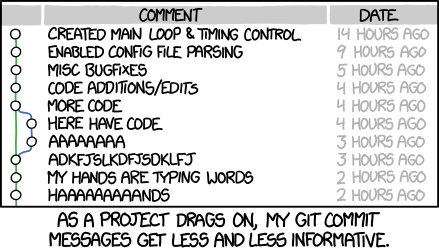
\includegraphics[width=4in]{git_commit.png}
\end{frame}

\begin{frame}{Subversion at NCAR}
CISL will stop hosting Subversion by Oct 1, 2016.
\end{frame}


\section{git}

\subsection{Distributed revision control}
\begin{frame}{git is distributed}
  \begin{enumerate}
    \item no central repo (but we can act like it)
    \item each repo is self-contained (though might not have everything)
    \item can do work locally and choose what to share to others
  \end{enumerate}
  \begin{center}
    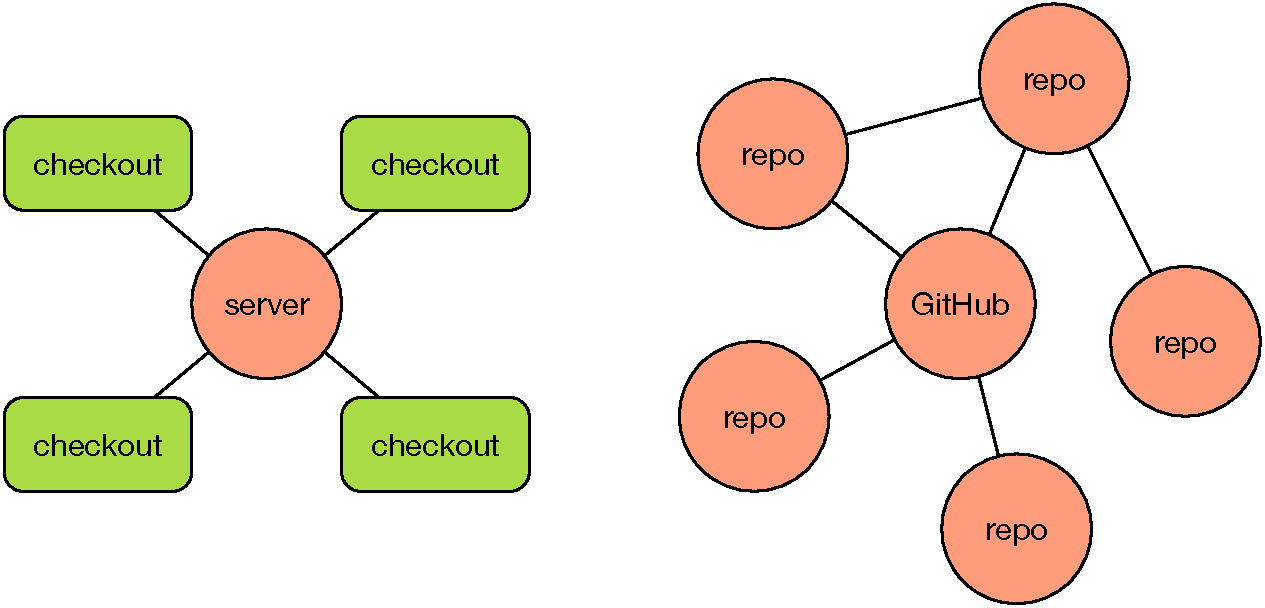
\includegraphics[width=3in]{drc.pdf}
  \end{center}
\end{frame}

\subsection{Getting code}
\begin{frame}[fragile]
  \frametitle{Cloning a repo}
  \begin{lstlisting}
git clone https://github.com/ncar-mlso/comp-utilities.git
git clone git@github.com:mgalloy/test.git
  \end{lstlisting}
\end{frame}

\subsection{Normal workflow}

\subsection{Reverting changes}


\begin{frame}{Resources}
  \begin{itemize}
    \item Just starting
      \begin{itemize}
        \item https://try.github.io/
        \item https://www.atlassian.com/git/tutorials/
      \end{itemize}
    \item Full reference
      \begin{itemize}
        \item Pro Git book: http://git-scm.com/book
      \end{itemize}
  \end{itemize}
\end{frame}

\section{GitHub}
\subsection*{}

\begin{frame}{Features}
  \begin{itemize}
    \item browsing files, commits, branches, tags, etc.
    \item issues tracker
    \item wiki pages (actually another git repo)
    \item social: watch/star repos, follow people
  \end{itemize}
\end{frame}

\begin{frame}{OS clients}
The GitHub client applications can handle non-GitHub repos as well.

\vspace{1em}

Get the appropriate client here:
  \begin{itemize}
    \item https://mac.github.com
    \item https://windows.github.com
  \end{itemize}
Sorry Linux! (The command line is better anyway.)
\end{frame}

\begin{frame}{OS clients}
  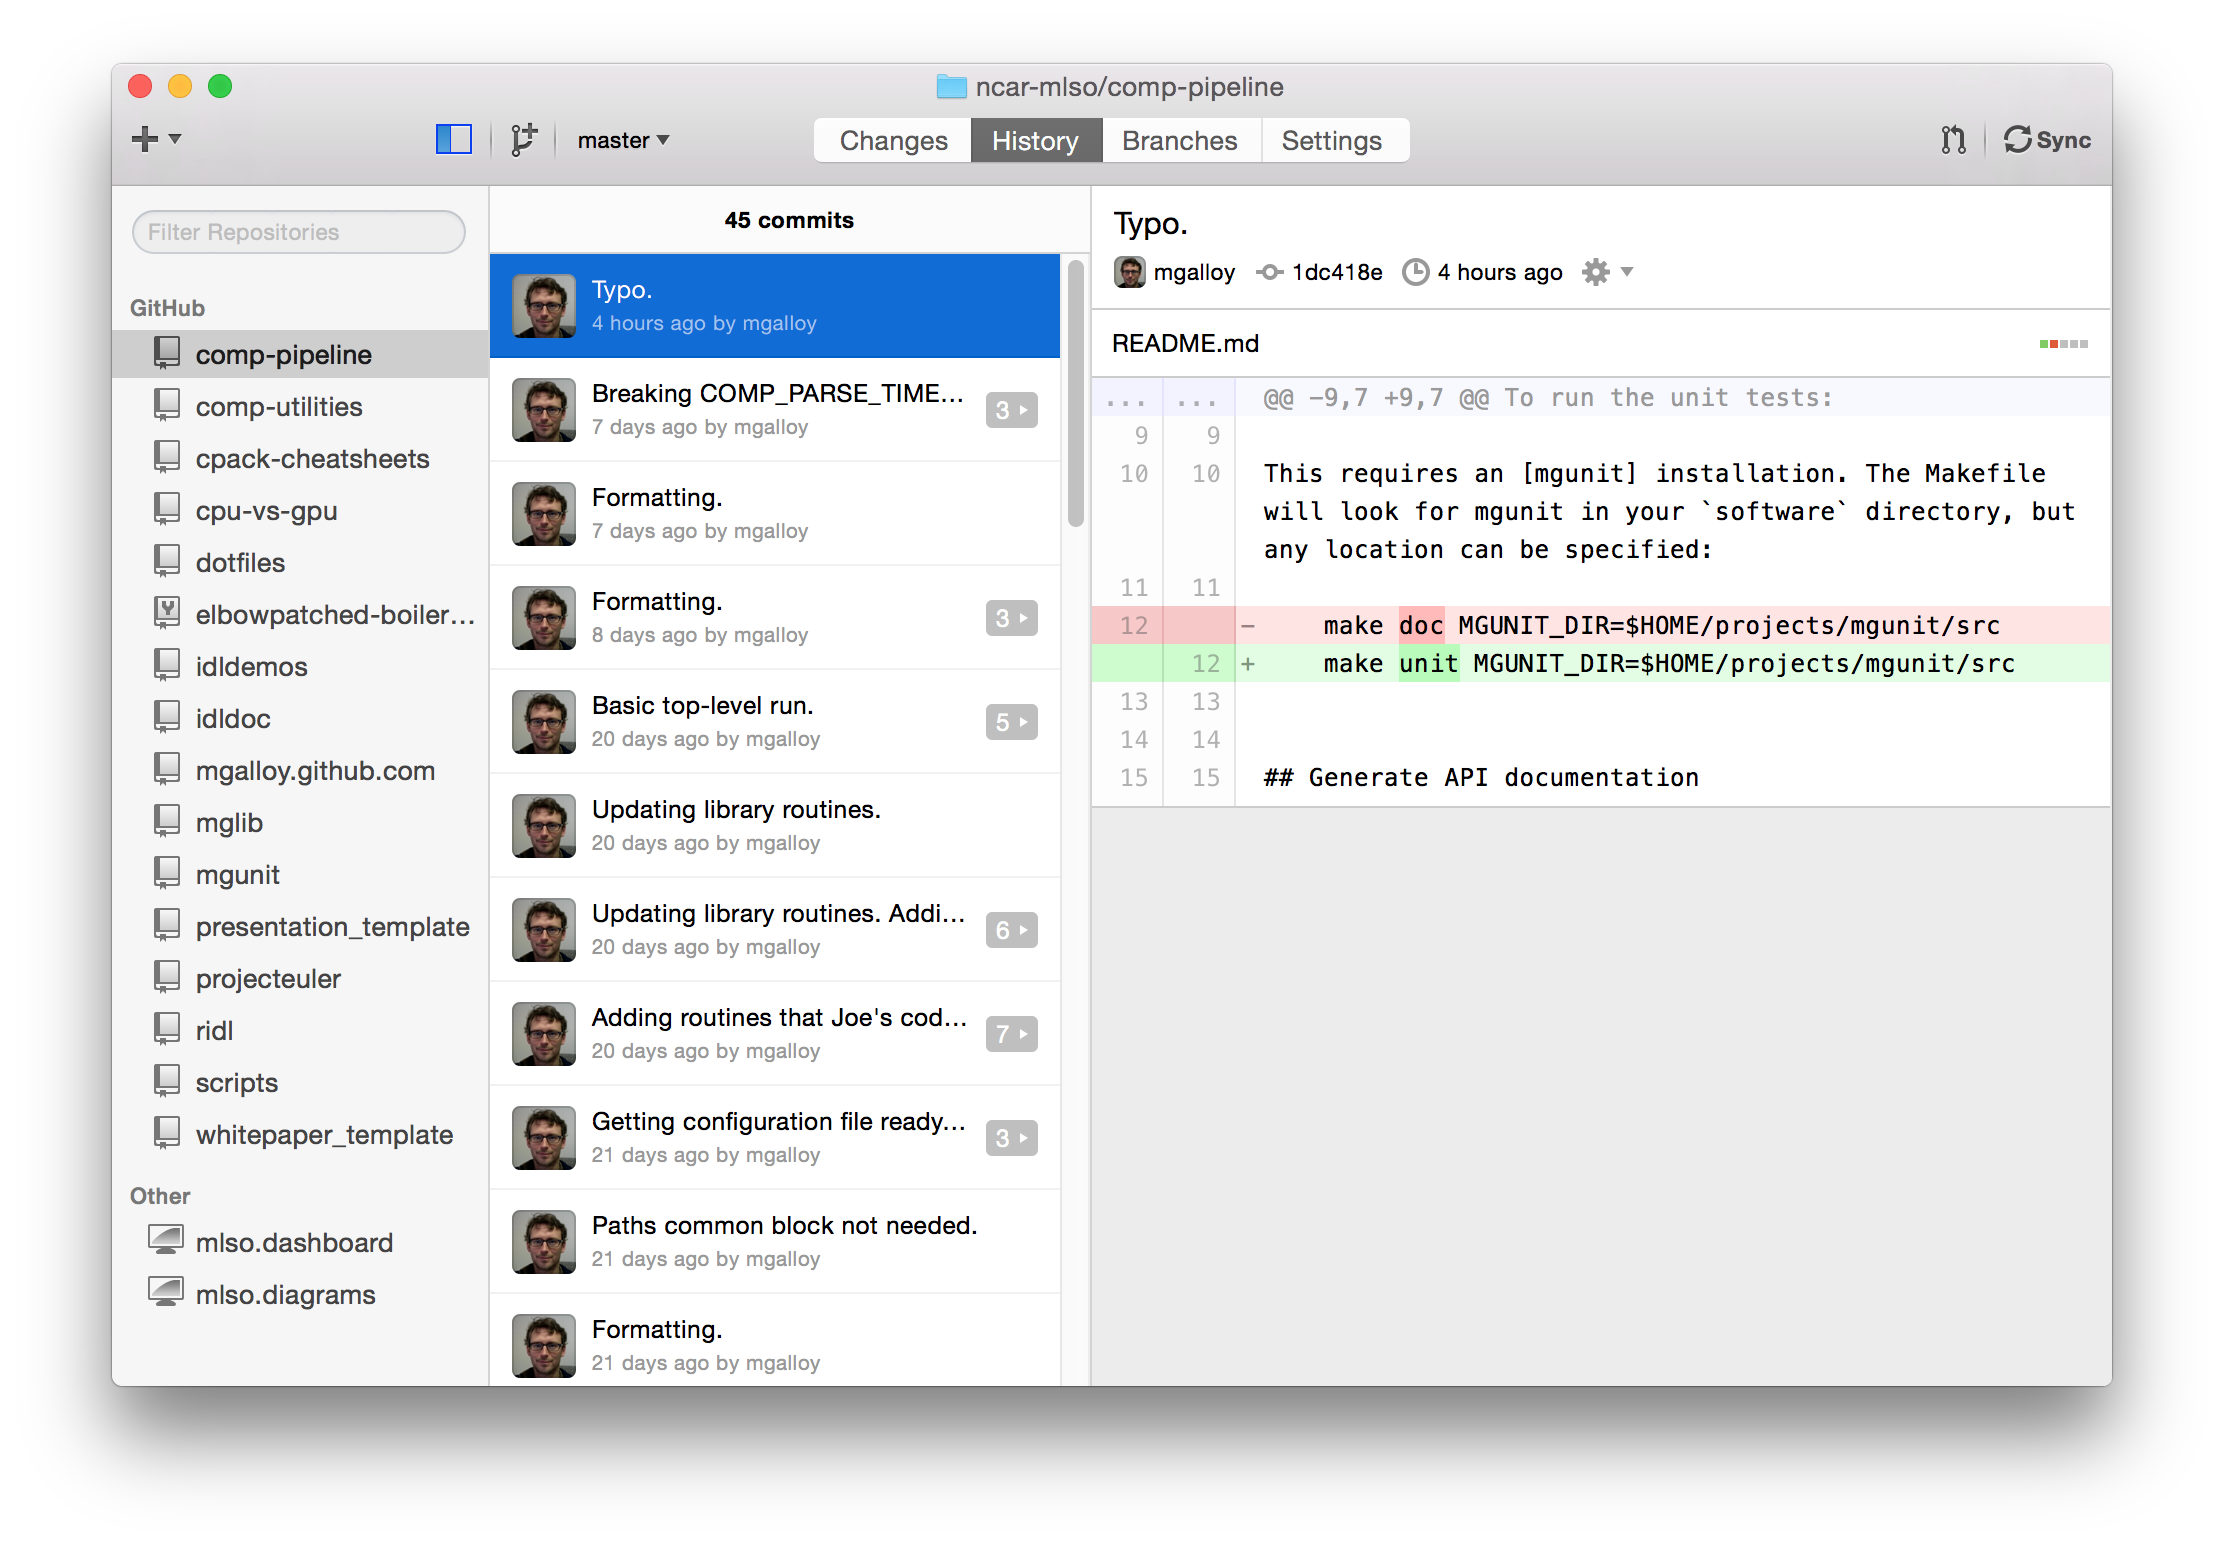
\includegraphics[width=4in]{mac-client.png}
\end{frame}


\section{Conclusion}
\subsection*{}

\begin{frame}{Conclusion}
  \begin{enumerate}
    \item While git is more powerful than Subversion, you can use it like Subversion
    \item GitHub provides an easy browser with social integration and other features such as issue tracker and wiki
  \end{enumerate}
\end{frame}

\begin{frame}{Thanks!}
  \begin{center}{\huge Thanks!}\end{center}
  \begin{itemize}
    \item {\tt mgalloy@ucar.edu}
  \end{itemize}
\end{frame}



\end{document}
